\begin{figure*}[htbp]
    \centering
    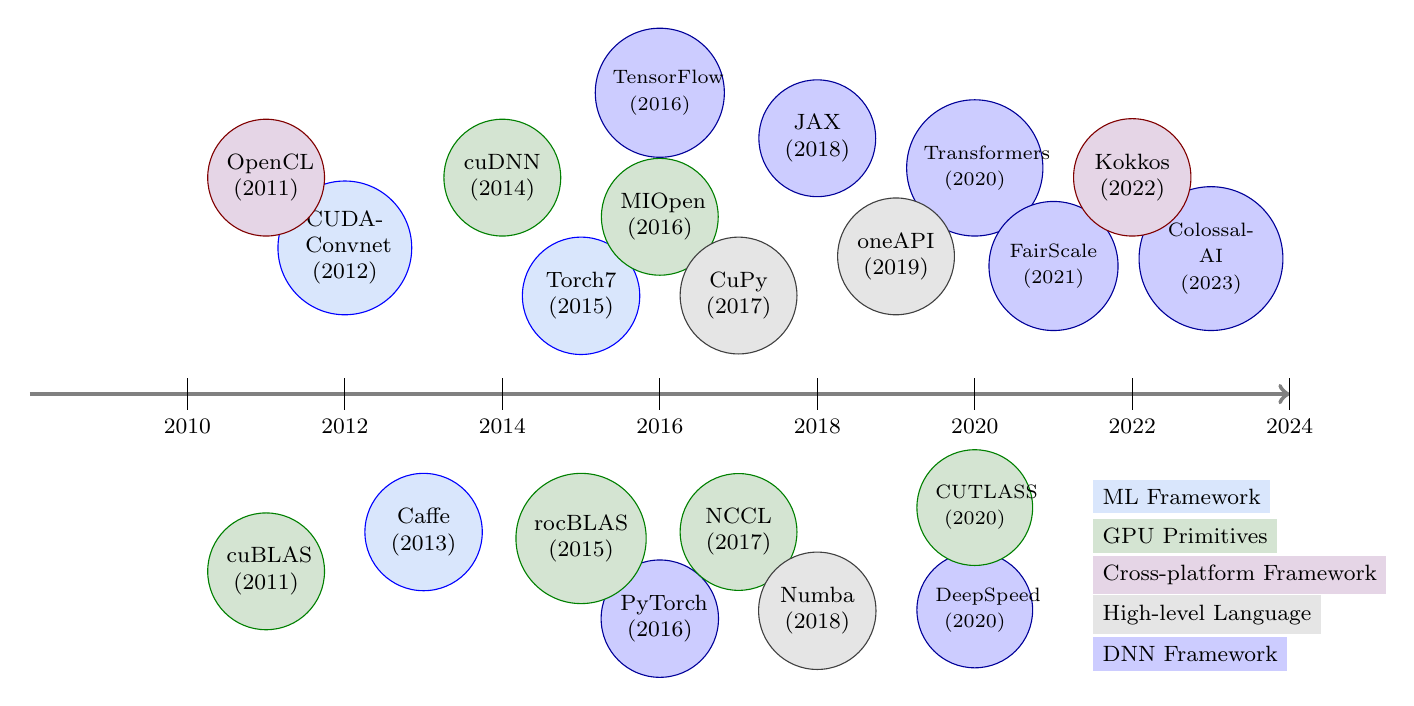
\begin{tikzpicture}[
        timeline/.style={
            ->,
            ultra thick,
            draw=gray
        },
        event/.style={
            circle,
            fill=blue!20,  % Hex: #d9e6fc
            draw=blue!60!black,
            text width=1cm,
            align=center,
            font=\footnotesize
        },
        levent/.style={
            circle,
            fill=blue!20,  % Hex: #d9e6fc
            draw=blue!60!black,
            text width=1.2cm,
            align=center,
            font=\footnotesize
        },
        llevent/.style={
            circle,
            fill=blue!20,  % Hex: #d9e6fc
            draw=blue!60!black,
            text width=1.3cm,
            align=center,
            font=\footnotesize
        },
        core/.style={
            circle,
            fill={rgb,255:red,212; green,228; blue,210},  % Hex: #d4e4d2
            draw=green!50!black,
            text width=1cm,
            align=center,
            font=\footnotesize
        },
        lcore/.style={
            circle,
            fill={rgb,255:red,212; green,228; blue,210},  % Hex: #d4e4d2
            draw=green!50!black,
            text width=1.2cm,
            align=center,
            font=\footnotesize
        },
        framework/.style={
            circle,
            fill={rgb,255:red,229; green,213; blue,230},  % Hex: #e5d5e6
            draw=red!50!black,
            text width=1cm,
            align=center,
            font=\footnotesize
        },
        language/.style={
            circle,
            fill=gray!20,
            draw=gray!50!black,
            text width=1cm,
            align=center,
            font=\footnotesize
        },
        eventg/.style={
            circle,
            fill={rgb,255:red,217; green,230; blue,252},
            draw=blue,
            text width=1cm,
            align=center,
            font=\footnotesize
        },
        leventg/.style={
            circle,
            fill=blue!20,
            draw=blue,
            text width=1.2cm,
            align=center,
            font=\footnotesize
        },
        lleventg/.style={
            circle,
            fill=blue!20,
            draw=blue,
            text width=1.3cm,
            align=center,
            font=\footnotesize
        },
        nvidia/.style={
            circle,
            fill=green!20,
            draw=green!50!black,
            text width=1cm,
            align=center,
            font=\footnotesize
        },
        amd/.style={
            circle,
            fill=red!20,
            draw=red!50!black,
            text width=1cm,
            align=center,
            font=\footnotesize
        },
        lamd/.style={
            circle,
            fill=red!20,
            draw=red!50!black,
            text width=1.2cm,
            align=center,
            font=\footnotesize
        },
        cross/.style={
            circle,
            fill=gray!20,
            draw=gray!50!black,
            text width=1cm,
            align=center,
            font=\footnotesize
        }
    ]
        % Main timeline
        \draw[timeline] (-2,0) -- (14,0);
        
        % Time markers
        \foreach \x/\year in {0/2010,2/2012,4/2014,6/2016,8/2018,10/2020,12/2022,14/2024} {
            \draw (\x,-0.2) -- (\x,0.2);
            \node[below] at (\x,-0.2) {\footnotesize \year};
        }
        
        % Original events
        \node[eventg, above] at (2,1) {CUDA-Convnet (2012)};
        \node[eventg, below] at (3,-1) {Caffe (2013)};
        \node[eventg, below] at (5,2) {Torch7 (2015)};
        

        
        % New DL framework events
        \node[levent, above] at (6,3) {{\scriptsize TensorFlow (2016)}};
        \node[event, below] at (6,-2.1) {PyTorch (2016)};
        \node[event, above] at (8,2.5) {JAX (2018)};
        \node[llevent, above] at (10,2) {{\scriptsize Transformers (2020)}};
        \node[event, below] at (10,-2) {{\scriptsize DeepSpeed (2020)}};
        \node[levent, above] at (11,0.8) {{\scriptsize FairScale (2021)}};
        \node[levent, above] at (13,0.8) {{\scriptsize Colossal-AI (2023)}};
        
        % ============== GPU ==============
        % Core technologies
        \node[core, above] at (1,-3) {cuBLAS (2011)};
        \node[core, above] at (4,2) {cuDNN (2014)};
        \node[core, above] at (7,-2.5) {NCCL (2017)};
        \node[core, below] at (10,-0.7) {{\scriptsize CUTLASS (2020)}};
        \node[lcore, below] at (5,-1) {rocBLAS (2015)};
        \node[core, below] at (6,3) {MIOpen (2016)};
        
        % Framework solutions
        \node[framework, above] at (1,2) {OpenCL (2011)};
        \node[framework, above] at (12,2) {Kokkos (2022)};
        
        % Language tools
        \node[language, below] at (7,2) {CuPy (2017)};
        \node[language, below] at (8,-2) {Numba (2018)};
        \node[language, above] at (9,1) {oneAPI (2019)};
        
        % ============== Legend ==============
        % Type color coding
        \node[draw=none, fill={rgb,255:red,217; green,230; blue,252}, right] at (11.5, -1.3) {\footnotesize ML Framework};  % Hex: #d9e6fc
        \node[draw=none, fill={rgb,255:red,212; green,228; blue,210}, right] at (11.5, -1.8) {\footnotesize GPU Primitives};  % Hex: #d4e4d2
        \node[draw=none, fill={rgb,255:red,229; green,213; blue,230}, right] at (11.5, -2.3) {\footnotesize Cross-platform Framework};  % Hex: #e5d5e6
        \node[draw=none, fill=gray!20, right] at (11.5, -2.8) {\footnotesize High-level Language};
        \node[draw=none, fill=blue!20, right] at (11.5, -3.3) {\footnotesize DNN Framework};
    \end{tikzpicture}
    \caption{Timeline of Major GPU Programming Libraries and Frameworks}
    \label{fig:gpu_timeline}
\end{figure*} 